%-------------------------------------------------------------------------------
%-------------------------------------------------------------------------------
%-------------------------------------------------------------------------------
\chapter{Zéros de fonctions}\label{chap:zero}
%-------------------------------------------------------------------------------
%-------------------------------------------------------------------------------
\thispagestyle{empty}

Un des problèmes numériques les plus connus est celui de la résolution des équations : 
on se donne un équation sous la forme $f(x) = 0$ est on cherche, une valeur de $x$, $x_0$, telle que $f(x_0)=0$. Dans la suite on nommera {\bf zéro} de $f$ une telle valeur.

On voit très vite qu'on a besoin de préciser le contexte :
\begin{itemize}
    \item un zéro doit-il appartenir à un ensemble donné ?
    \item cherche-ton un zéro ou tous les zéros ?
    \item sait-on s'il existe un zéro, s'il est unique ?
\end{itemize}

On supposera ici que la fonction $f$ est définie sur une partie de $\R$ et à valeurs réelles.

Ce problème est au cœur de nombreux résultats mathématiques :

\begin{itemize}
    \item existence d'un zéro : théorème de Rolle
    \item unicité du zéro : injectivité
    \item résolution avec extractions de racines dans le cas des polynômes de degré 2, puis 3, puis 4
    \item fonctions réciproques, par exemple $\arcsin(a)$ est l'unique solution de $\sin(x) = a$ sur $[-\pi/2;\pi/2]$
    \item \dots
\end{itemize}

Résoudre une équation est parfois considéré comme la recherche d'une expression du zéros à l'aide d'un ensemble de fonctions considérées comme connues. On considère plutôt les équations de la forme $f(x)=a$ avec $f$ bijective et on cherche la fonction $f^{-1}$. Une forme d'expertise en mathématique serait alors de savoir résoudre le plus possible d'équations. 

\medskip

Cependant si l'objectif est d'avoir un valeur numérique du zéro, on n'aura pratiquement jamais une valeur exacte car les fonction utilisées ne sont exactement calculables. L'objectif de ce chapitre sera, inversement, de calculer une valeur approchée du zéro pour un ensemble très général d'équations, contenant celles que l'on estime résolubles mathématiquement.

\medskip

On se place dans le cadre des fonctions continues sur un intervalle $[a;b]$ et on cherche des approximations d'une solution de $f(x)=0$ ; on suppose que $f$ admet au moins un zéro sur $[a;b]$. 

Il sera souvent utile de se restreindre à un intervalle dans lequel on a prouvé que la fonction admet une racine unique : la figure \ref{grf:unZero} représente ce type de cas.

Nous étudions dans ce chapitre deux méthodes :
\begin{enumerate}
  \item la méthode de dichotomie est valable pour les fonctions continues et donne une approximation dans tous les cas où on a su encadrer un zéro de la fonction,
  \item la seconde méthode, de Newton, nécessite d'avoir une fonction dérivable et peut ne pas donner d'approximation. Cependant, en cas de convergence, elle est très rapide. De plus elle se généralise au cas de recherche de zéros d'une fonctions de $\R^n$ vers $\R^n$.
\end{enumerate}
%-------------------------------------------------------------------------------
\begin{figure}[ht]
  \begin{center}
      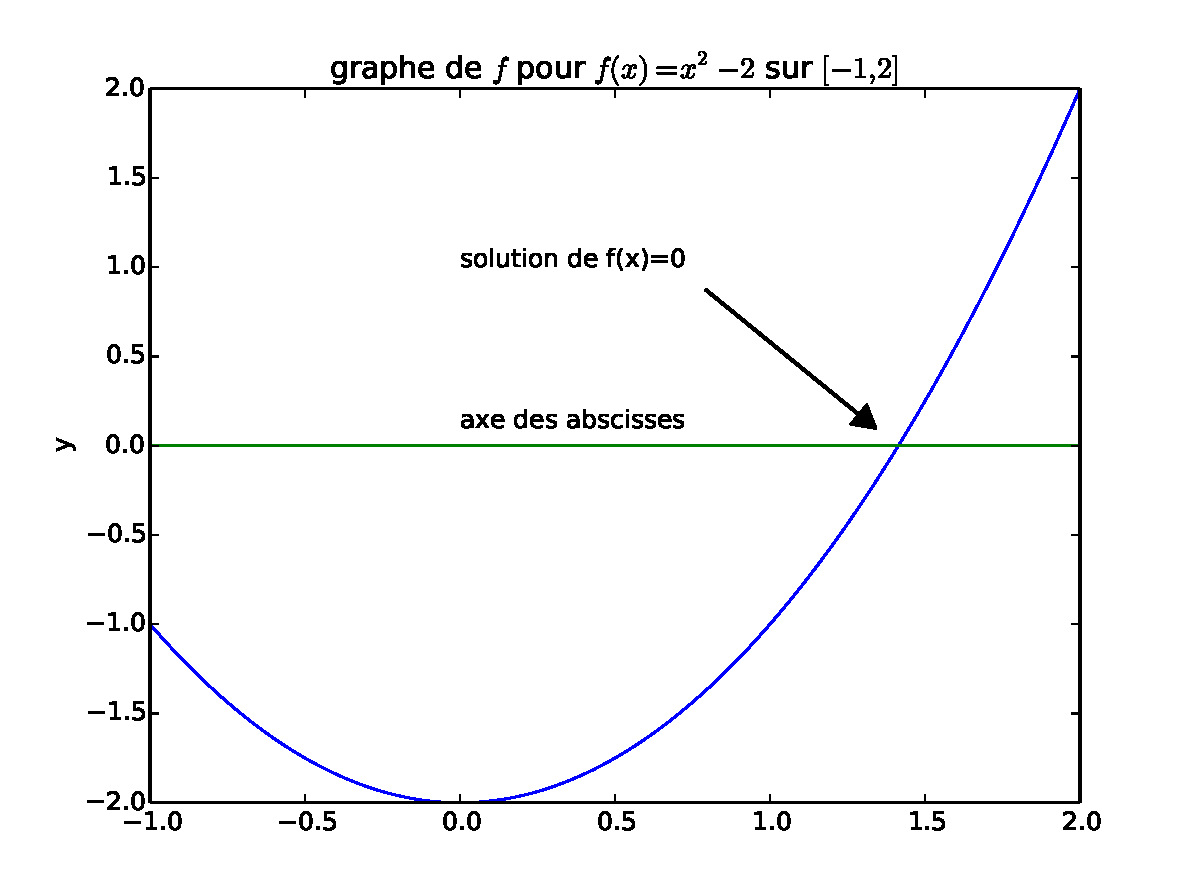
\includegraphics[scale=0.4]{13_zero.pdf}
      \caption{\label{grf:unZero} Fonction à zéro unique}
  \end{center}
\end{figure}
%-------------------------------------------------------------------------------
%-------------------------------------------------------------------------------
%-------------------------------------------------------------------------------
\section{Méthode de dichotomie}
%-------------------------------------------------------------------------------
%-------------------------------------------------------------------------------
\subsection{La méthode mathématique}
%-------------------------------------------------------------------------------
On travaille ici sur un intervalle $I=[a,b]$ en supposant $a<b$ et $f(a)f(b) <0 $.

L'idée est d'utiliser le théorème des valeurs intermédiaires pour diminuer la largeur de l'intervalle d'étude par 2.
%-------------------------------------------------------------------------------
\begin{enumerate}
\item On pose $c = \frac{a+b}{2}$ et on calcule $f(c)$,
\item Si $f(a) f(c) <0 $, alors $f$ s'annule sur $]a; c[$.
\item Sinon $f$ s'annule sur $[c; b[$ et on étudie sur $ [c,b]$
\end{enumerate}
%-------------------------------------------------------------------------------

On peut alors itérer cette idée en notant $a_{0}=a$ et $b_{0}=b$  et en construisant trois suites $(a_n)$, $(b_n)$ et $(c_n)$ de la façon suivante :
%-------------------------------------------------------------------------------
\begin{enumerate}
\item on pose $c_n = \frac 1{2}(a_n+b_n)$ et on calcule $f(c_n)$,
\item si $f(a_n) f(c_n) \le 0 $, alors on définit $a_{n+1} = a_n$ et $b_{n+1}=c_n$,
\item sinon on définit $a_{n+1} = c_n$ et $b_{n+1}=b_n$.
\end{enumerate}
%-------------------------------------------------------------------------------
\begin{figure}[ht]
  \begin{center}
      \begin{tikzpicture}[xscale=2]
      \draw[thick, ->] (-1.3, 0) --(2.3, 0);
      \draw[thick, ->] (0, -2.3) --(0, 2.3);
      \draw [samples=100,domain=-1:2] plot({\x},{\x*\x-2});
      \draw[dotted] ( -1  , 0) node[above]{$a_0$} -- +(0, -1);
      \draw[dotted] (  2  , 0) node[below]{$b_0$} -- +(0,  2);
      \draw[dotted] (0.5  , 0) node[above]{$c_0$} -- +(0, -1.75);
      \draw[dotted] (1.25 , 0) node[above]{$c_1$} -- +(0, -0.4375);
      \draw[dotted] (1.625, 0) node[below]{$c_2$} -- +(0,  0.6406);
      \end{tikzpicture}
  \caption{\label{grf:c0c1c2} Premières valeurs de $c_n$}
  \end{center}
\end{figure}
%-------------------------------------------------------------------------------
Pour l'exemple initial on a représenté, dans la figure \ref{grf:c0c1c2}, les premières valeurs de $c_n$.

On a $a_1=c_0$, $a_2=a_3=c_1$, $b_0=b_1=b_2$ et $b_3=c_2$.

%-------------------------------------------------------------------------------
  \begin{thm}
Les deux suites  $(a_n)_{n\in \N}$ et $(b_n)_{n\in \N}$ sont adjacentes et leur limite commune est un zéro de $f$.

De plus on a $\displaystyle b_n - a_n= \frac{b_0-a_0} {2^n}$.\end{thm}
%-------------------------------------------------------------------------------
\subsection{Algorithme}
%-------------------------------------------------------------------------------
%-------------------------------------------------------------------------------
\begin{lstlisting}[caption = {Calcul d'un zéro par dichotomie}]
def dichotomie(f, a, b, epsilon):
    """Entrées : un fonction, 3 flottants
       Requis  : a < b, f s'annule sur [a; b],  epsilon > 0
       Sortie  : une valeur approchée de f sur [a; b] 
                 à epsilon près"""
    while b - a > epsilon:   # precision non atteinte
        c = (a+b)/2          # calcul du milieu de a et b
        if f(a) * f(c) <= 0:
            b = c            # on change l'extremite droite
        else:
            a = c            # on change l'extremite gauche
    return (a+b)/2
\end{lstlisting}
%-------------------------------------------------------------------------------
%-------------------------------------------------------------------------------
\subsection{Analyse de l'algorithme}
%-------------------------------------------------------------------------------
%-------------------------------------------------------------------------------
\subsubsection{L'algorithme termine}
%-------------------------------------------------------------------------------
  Il faut prouver que l'on sort de la boucle \type{while}.
  
  On a $\displaystyle b_n - a_n= \frac{b_0-a_0} {2^n}$. Ainsi $\lim\limits_{n\rightarrow +\infty} b_n - a_n=0$ donc $b_n - a_n \le \varepsilon$ pour $n$ supérieur à un entier $N$.
  
  \type{b - a} vaut $b_n - a_n$ après $n$ passages dans la boucle donc la condition \type{b - a > epsilon} est fausse pour $n\ge N$ : on est sûr que l'on n'itère la boucle qu'un nombre fini de fois. 
%-------------------------------------------------------------------------------
\subsubsection{L'algorithme est correct}
%-------------------------------------------------------------------------------
Il faut prouver qu'il existe un réel $r$ tel que $f(r=0)$ et $|r-c| < \varepsilon$ si $c$ est la valeur renvoyée par \type{ dichotomie(f, a, b, epsilon)}. 
La limite commune, $r$,  des suites $(a_n)_{n\in \N}$ et $(b_n)_{n\in \N}$  est un zéro de $f$ et vérifie $a_n\le r \le b_n$ on a donc  $\displaystyle a-\frac{a+b}2 \le r - \frac{a+b}2 \le b - \frac{a+b}2$ à chaque étape d'où $\displaystyle \bigl|r-\frac{a+b}2\bigr|\le \frac{b-a}2\le \frac 12\varepsilon < \varepsilon$ à la sortie de la fonction. 
%-------------------------------------------------------------------------------
\subsubsection{Nombre d'opérations}
%-------------------------------------------------------------------------------
On peut déterminer le nombre de parcours de la boucle en cherchant le premier entier $k$ tel que $\displaystyle \frac{b-a}{2^k} \le \epsilon $. 
On a alors $\displaystyle \frac{b-a}{\epsilon} \le 2^k$ c'est-à-dire $\displaystyle \ln\bigl(\frac{b-a}{\epsilon}\bigr) \le k*\ln(2)$.
Il suffit donc  $\displaystyle k= \bigl\lfloor \frac{\ln(\frac{b-a}{\epsilon})}{\ln(2)}\bigr\rfloor + 1 $ opérations à effectuer pour avoir une valeur approchée de $r$ à $\epsilon$ près.
%-------------------------------------------------------------------------------

\newpage
%-------------------------------------------------------------------------------
\subsection{Remarques}
%-------------------------------------------------------------------------------
%-------------------------------------------------------------------------------
\begin{itemize}
  \item En pratique, on ne connaît pas toujours la fonction $f$ en tout point mais on dispose seulement d'un nombre fini de ses valeurs (penser par exemple à l'acquisition d'un son numérique) sous la forme d'une liste $y=[y_0,y_1,\cdots ,y_{n-1}]$ de longueur $n$ qui représente la liste des valeurs prises par la fonction.
  
  Si on suppose la fonction croissante (ou décroissante), une bonne approximation de la racine $r$ sera alors $y_q$ avec $q$ le premier entier tel que $y_q>0$
($y_{q-1}$ serait aussi une bonne approximation sans qu'on puisse vraiment les départager).

On est donc amené à chercher, dans une liste ordonnée, le premier terme qui dépasse $0$. Une méthode coûteuse serait de parcourir la liste jusqu'à trouver un terme positif, on  utilisera plutôt une dichotomie comme on l'a vu dans le cours sur les recherches dans des listes triées.
%-------------------------------------------------------------------------------
\item Le fait que l'algorithme termine est prouvé mathématiquement mais il faut tenir compte des erreurs dues à l'usage des flottants. Il vaut mieux éviter des valeur de \type{epsilon} trop petite pour que le calcul de \type{(a+b)/2} donne un résultat distinct de \type{a}. Dans la pratique on choisira $\varepsilon$ supérieur à $10^{-12}$ fois l'ordre de grandeur de $a$ et $b$.
%-------------------------------------------------------------------------------
\item La valeur renvoyée n'est correcte que si les erreurs d'arrondi ne perturbent pas les tests.

En effet un test de comparaison à 0 n'est pas fiable pour des flottants.

Par exemple la fonction $f$ : $\displaystyle x \mapsto \sin(x) - x + \frac{x^3}{6} + \frac{x^5}{120}$ est plate autour de son unique racine et le signe de $f(x)$ n'est pas bien calculé pour des valeurs de $x$ proches de 0.
%-------------------------------------------------------------------------------
\begin{figure}[ht]
  \begin{center}
      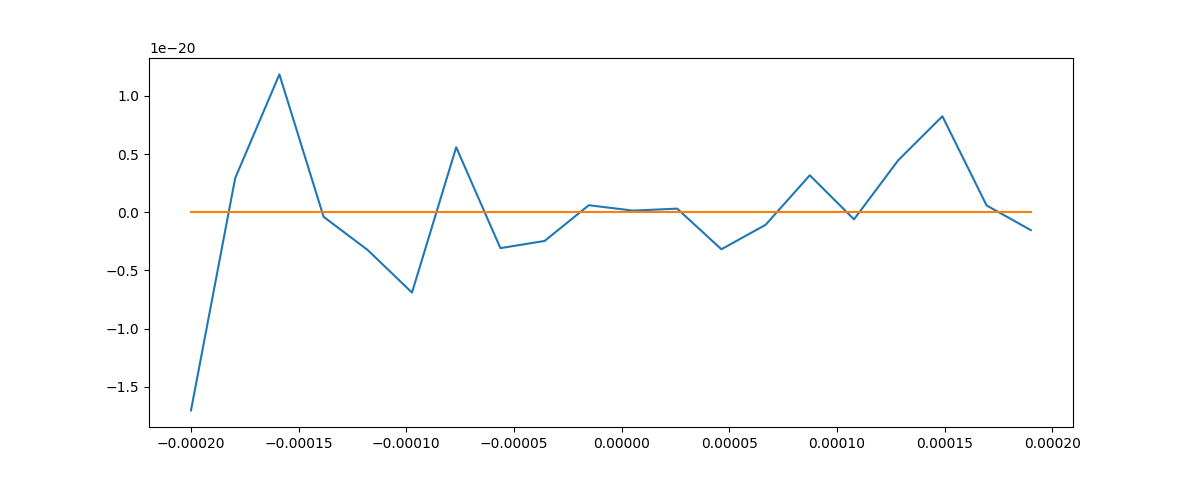
\includegraphics[scale=0.5]{13_fauxSigne}
      \caption{\label{grf:fauxSigne} Signes non exacts de $x\mapsto \sin(x) - x + \frac{x^3}{6} + \frac{x^5}{120}$}
  \end{center}
\end{figure}
%-------------------------------------------------------------------------------

\type{Dichotomie(f, -0.4, 0.6, 1e-6)} renvoie \type{0.000207996} qui n'est pas une valeur approchée à $\varepsilon$ près.
\end{itemize}
%-------------------------------------------------------------------------------
\newpage
%-------------------------------------------------------------------------------
\section{Méthode de Newton}
%-------------------------------------------------------------------------------
%-------------------------------------------------------------------------------
\subsection{La méthode}
%-------------------------------------------------------------------------------
On suppose pour cette méthode $f$ de classe ${\cal C}^1$ sur un intervalle $I$ 

avec $f$ s'annulant en au moins un point de $I$. 

On part de $x_0\in I$ ; la tangente à la courbe représentative de $f$ en $\bigl(c,f(c)\bigr)$ recoupe l'axe des abscisses en un point $(x_1,0)$. 
Si $x_1$ appartient à $I$, on réitère le procédé avec le point $(x_1,f(x_1))$. 

On continue ainsi (quand c'est possible).

On remarque dans l'exemple de la figure \ref{grf:newton} que $x_2$ est proche d'une racine. Dans le graphe la tangente en $\bigl(x_2, f(x_2)\bigr)$ est indiscernable de la courbe donc $x_3$ sera une excellente approximation.
%-------------------------------------------------------------------------------
\begin{figure}[ht]
  \begin{center}
      \begin{tikzpicture}[xscale=2]
      \draw[thick, ->] (-1.3, 0) --(2.8, 0);
      \draw[thick, ->] (0, -2.3) --(0, 3.8);
      \draw [samples=100,domain=-1:2.5] plot({\x},{\x*\x-2});
      \draw[dotted] (0.5, 0) node[above]{$x_0$} -- +(0, -1.75);
      \draw[dashed](0, -2.25) -- (3, 0.75);
      \draw[dotted] (2.25, 0) node[below]{$x_1$} -- +(0, 3.0625);
      \draw[dashed](1, -2.5625) -- (2.5, 4.1875);
      \draw[dotted] (1.566, 0) node[below]{$x_2$} -- +(0, {1.566*1.566-2});
       \end{tikzpicture}
  \caption{\label{grf:newton} 2 étapes dans la méthode de Newton}
  \end{center}
\end{figure}
%-------------------------------------------------------------------------------
\medskip

La tangente en $(c,f(c))$, $T_c$, admet pour équation $y - f(c) = f'(c) (x-c) $.

La relation de récurrence qui définit la suite $(x_n)$ est donc

\[ x_0=c \text{ et  } \forall n \in \mathbf{N}, \quad x_{n+1} = x_n -\frac{f(x_n)}{f'(x_n)} \]
%-------------------------------------------------------------------------------
\subsection{Convergence}
%-------------------------------------------------------------------------------
La convergence est démontrable dans un cas particulier.
%-------------------------------------------------------------------------------
\begin{thm}
$f$ est de classe ${\cal C}^2$ sur $[a; b]$ avec
\begin{itemize}
  \item $f'$ et $f''$ de signe constant
  \item $f(a).f(b) < 0$.
\end{itemize}
Si $x_0 = b$ quand $f'$ et $f''$ sont de même signe ou $x_0 = a$ pour $f'$ et $f''$ de signe opposés 

alors la suite $(x_n)$ définie par
$\displaystyle x_{n+1}=x_n -\frac{f(x_n)}{f'(x_n)}$ est bien définie et monotone dans $[a;b]$.

Cette suite converge vers l'unique racine de $f$ dans $[a;b]$.

On a, de plus $x_{n+1} - x_n \sim r - x_n$ quand n tend vers l'infini
et $\displaystyle |r - x_{n+1}| \le \frac {M_2}{m_1} (r - x_n)^2=K(r - x_n)^2$ pour $M_2$ majorant de $|f''|$ sur $[a;b]$ et $m_1$ minorant de $|f'|$ sur $[a;b]$.
\end{thm}
%-------------------------------------------------------------------------------
% Il y a 4 cas possibles pour les signes : on supposera ici qu'on a $f'(x) > 0$, $f''(x) > 0$ et $f(a) < 0 < f(b)$.

% $f$ s'annule en un point unique, noté $r$, et on a $f(x)< 0$ pour $x\in[a;r[$ et $f(x)> 0$ pour $x\in]r;b]$.

% On choisit donc $x_0=b$.
% %-------------------------------------------------------------------------------
% \begin{enumerate}
%   \item On suppose que $x_n$ est bien défini et appartient à $]r; b]$. 
  
%   On a $f'(x_n) > 0$ donc $\displaystyle x_{n+1}=x_n -\frac{f(x_n)}{f'(x_n)}$ est bien défini.
  
%   $f$ et $f'$ sont positives donc $x_{n+1} < x_n \le b$.
  
%   La formule de Taylor en $x_n$ donne $\displaystyle f(x) = f(x_n) + (x-x_n)f'(x_n) + \int_{x_n}^x (x-t)f''(t) dt$. 
  
%   Pour $x = r$ on obtient $\displaystyle f(r)= 0 =f(x_n) + (r-x_n)f'(x_n) + \int_{x_n}^r (r-t)f''(t) dt$.
  
%   Comme on a $r< x_n$ on a $r-t < 0$ pour $t\in ]r; x_n[$ d'où comme $f''$ est strictement positive et $x_n> r$, $\displaystyle \int_{x_n}^r (r-t)f''(t) dt > 0$.
  
%   On en déduit qu'on a $f(x_n) + (r-x_n)f'(x_n)< 0$ d'où $\displaystyle r < x_n - \frac{f(x_n)}{f'(x_n)}=x_{n+1}$.
  
%   On a donc prouvé, par récurrence que $x_n \in ]r; b]$ pour tout $n$ avec $x_n < x_{n+1}$.
%  %-------------------------------------------------------------------------------
%   \item La suite $(x_n)$ est décroissante minorée par $r$ donc converge vers une limite $r'$. 
  
%   Comme les fonctions sont continues le passage à la limite de $\displaystyle x_{n+1}=x_n -\frac{f(x_n)}{f'(x_n)}$ donne $\displaystyle r' = r' -\frac{f(r')}{f'(r')}$ d'où $f(r')=0$ puis $r=r'$.
%   La suite $(x_n)$ converge vers $r$.
% %-------------------------------------------------------------------------------
% \item On a $\displaystyle x_{n+1}-x_n=-\frac{f(x_n)}{f'(x_n)}=\frac{f(r)-f(x_n)}{f'(x_n)}\sim \frac{(r-x_n)f'(x_n)}{f'(x_n)}=r-x_n$.

% Ainsi l'approximation faite en approchant $r$ par $x_n$ est de l'ordre de $x_{n+1}-x_n$ cela permet de donner une condition d'arrêt pour l'algorithme.
% %-------------------------------------------------------------------------------
% \item Des formules de Taylor en $r$ permettent d'écrire

% \begin{eqnarray*}
%   x_{n+1}-r 
%   &
%   x_n - r -\frac{f(x_n)}{f'(x_n)}= x_n - r -\frac{f(r)+(x_n-r) f'(r) + (x_n-r)^2\frac{f''(x_n)}2+(x_n-r)^2\varepsilon(x_n)}
% {f'(r) + (x_n-r)f''(r) + (x_n-r)\varepsilon_1(x_n)}
% \\ &
% \frac{(x_n-r)^2\frac{f''(x_n)}2+(x_n-r)^2\varepsilon(x_n)}{f'(r) + (x_n-r)f''(r) + (x_n-r)\varepsilon_1(x_n)}
% \sim \frac{(x_n-r)^2 f''(x_n)}{2f'(r)}
% \sim \frac{(x_n-r)^2 f''(r)}{2f'(r)}
% \end{eqnarray*}

% On peut donc majorer $|x_{n+1}-r| \le K|x_{n}-r|^2$ donc $|x_n-r| \le K|x_0-r|^{2^n}$.
\newpage
%-------------------------------------------------------------------------------
\begin{enumerate}
 \item Dans le cas général, il peut ne pas y avoir de convergence :
 
\begin{itemize}
 \item soit parce que $f'(x_n) = 0$, par exemple pour $f(x) = \frac{1-x}{x^2}$ et $x_0 = 2$
 
 \item soit parce que la valeur de $x_n$ n'appartient plus à un intervalle où on sait calculer $f$,
 
 par exemple pour $f(x) = 4\sqrt x -x$ et $x_0=1$
 
 \item soit parce que la suite n'admet pas de limite, par exemple pour $f$ : $x \mapsto \frac 1{27}\bigl(2x^3-3x^2-21x+11\bigr)$ et $x_0 = 2$. On trouve alors $x_1=-1$ puis $x_2 = 2$, la suite est 2-périodique.
%-------------------------------------------------------------------------------
  \begin{center}
      \begin{tikzpicture}[scale=3]
      \draw[thick, ->] (-1.3, 0) --(2.3, 0);
      \draw[thick, ->] (0, -1.3) --(0, 1.3);
      \draw [samples=100,domain=-1.1:2.1] plot({\x},{(2*\x*\x*\x-3*\x*\x-21*\x+11)/27});
      \draw[dotted] ( 2, 0) node[above]{$x_0=x_2$} -- +(0, -1);
      \draw[dotted] ( -1, 0) node[below]{$x_1$} -- +(0, 1);
      \draw[dashed] ( 2.3, -0.1)  -- (-1.3, 1.1);
      \draw[dashed] (-1.3, 0.1)  -- (2.3, -1.1);
      \end{tikzpicture}
  \end{center}
%-------------------------------------------------------------------------------
\end{itemize}
\item Si le zéro, $r$, de la fonction n'est pas un minimum ou un minimum, alors les conditions du théorème sont vérifiées dans un intervalle autour de $r$. Dans la pratique on pourra approcher un zéro par quelques étapes de dichotomie et on continuera  ensuite avec la méthode de Newton.
\item En effet, si on a $|x_0-r| \le \frac 1{2K}$, l'inégalité $|r - x_{n+1}| \le K(r - x_n)^2$ donne $\displaystyle |r - x_n|\le 1{K.2^{2^n}}$ : la convergence mathématique est très rapide, le nombre de chiffres exact double à chaque étape. Cela signifie que si $x_0$ est une valeur approchée à $10^{-1}$, il suffit de 4 étapes pour obtenir la précision maximale pour les flottants de $10^{-16}$.
\end{enumerate}
%-------------------------------------------------------------------------------
\subsection{Codage de la méthode de Newton}
%-------------------------------------------------------------------------------
La fonction calcule $x_n$ en prenant en paramètres $\epsilon$, $x_0$, $f$ et $f'$. On doit définir $f$ et $f'$ par des fonctions python car on ne sait pas calculer la dérivée de $f$ en Python.

L'équivalent $x_{n+1} - x_n \sim r - x_n$ du théorème permet de donner un critère de sortie de la boucle \type{while} sans connaître $r$.
%-------------------------------------------------------------------------------
\begin{lstlisting}[caption = {Calcul d'un zéro par la méthode de Newton}]
def Newton(x0, f, df, epsilon): 
    """Entrées : un réel, deux fonctions et un réel
       Requis : df est la dérivée de f, epsilon > 0
       Sortie : une valeur approchée d'un zéro de f"""
    x = x0
    difference = epsilon +1 # pour faire au moins un calcul
    while difference > epsilon:
        x_old = x
        x = x - f(x)/df(x)
        difference = abs(x - x_old)
    return x
\end{lstlisting}
%-------------------------------------------------------------------------------

\newpage
%-------------------------------------------------------------------------------
%-------------------------------------------------------------------------------
\section{\type{fsolve}}\label{sec:fsolve}
%-------------------------------------------------------------------------------
%-------------------------------------------------------------------------------
Le module \type{scipy} contient, dans la sous-bibliothèque \type{optimize} une fonction \type{fsolve} qui résout efficacement les équations. C'est la méthode à utiliser quand la résolution d'une équation est un outil d'un projet plus large.
%--------------------------------------------------------------------------
\begin{lstlisting}
from scipy.optimize import fsolve
\end{lstlisting}
%--------------------------------------------------------------------------
\begin{itemize}
\item \type{fsolve} reçoit pour paramètres une fonction $f$ dont on cherche un zéro et un valeur initiale autour de laquelle on cherche une solution.
\begin{lstlisting}
def f(x):
    return x**2 - 2
>>> fsolve(f, 1)
array([1.41421356])
\end{lstlisting}
%--------------------------------------------------------------------------
\item On remarque que la réponse est une liste (en fait un tableau \type{numpy}) avec un seul élément : on devra sortir la réponse.
\begin{lstlisting}
a = fsolve(f, 1)
zero = a[0]
\end{lstlisting}
\item La raison est que \type{fsolve} peut chercher un zéro d'une fonction de $\R^n$ vers $\R^n$
\begin{lstlisting}
def F(u):
    x, y = u
    return x + y - 3, x*y -2
>>> fsolve(F, (1, 1))
array([1., 2.])
\end{lstlisting}
%--------------------------------------------------------------------------
\item Si la fonction dont on recherche un zéro contient des paramètres on peut les définir lors de la résolution à l'aide de l'argument optionnel nommé par \type{args}.
\begin{lstlisting}
def g(x, a):
    return x**a -2 
>>> fsolve(g, 1, args = 2.5)
array([1.31950791])
\end{lstlisting}

\item On peut, par exemple, chercher un zéro d'un polynôme de degré 3 en donnant les coefficients.
\begin{lstlisting}
def poly3(x, a, b, c):
    return x**3 + a*x**2 + b*x + c 
>>> fsolve(poly3, 1, args = (1, 2, 3))
array([-1.2756822])
\end{lstlisting}
\end{itemize}
    


% %-------------------------------------------------------------------------------
% %-------------------------------------------------------------------------------
% \section{Autres méthodes}
% %-------------------------------------------------------------------------------
% %-------------------------------------------------------------------------------
% \subsection{Dichotomie dans une liste}
% %-------------------------------------------------------------------------------
% Une fonction $f$ est représentée par deux listes \type{X} et \type{Y} où

% \type{X} est une liste de valeurs, qu'on peut supposer régulièrement espacées

% \type{Y} est la liste des valeurs de $f$ aux points de \type{X} : \type{Y[i]} est la valeur de $f$ en \type{X[i]}.

% Les deux listes ont la même longueur.

% On suppose que $f$ est strictement monotone et change de signe. 
% %-------------------------------------------------------------------------------
% %-------------------------------------------------------------------------------
% \begin{Exercise}[label=exo:racineListe]
% Écrire un algorithme utilisant la méthode de dichotomie qui donne la valeur de \type{X[i]} telle que $f$ change de signe entre \type{X[i]} et\type{X[i+1]}.
% \end{Exercise}
% %-------------------------------------------------------------------------------
% \begin{Answer}
% \begin{lstlisting}
% def zeroListe(X, Y):
%     """ Entrées : 2 listes de même longueur
%         Requis : Y est strictement croissante et change de signe
%         Sortie : X(i] tel que Y[i] < 0 <= Y[i+1]"""
%     n = len(X)
%     a = 0
%     b = n - 1
%     while b - a > 1:
%         c = (a+b)//2
%         if Y[a]*Y[c] <= 0:
%             b = c
%         else:
%             a = c
%     return X[a]
% \end{lstlisting}
% \end{Answer}
% %-------------------------------------------------------------------------------
% %-------------------------------------------------------------------------------
% \subsection{Calcul de la dérivée}
% %-------------------------------------------------------------------------------
% Dans la méthode de Newton, on a vu qu'on a besoin de connaître la dérivée de la fonction. 

% Cette dérivée n'est pas toujours facile (et parfois impossible) à calculer.

% On peut alors tenter de remplacer la valeur $f'(x_n)$ par une valeur approchée.
% \medskip

% On sait que si une fonction $f$ est dérivable en un point $x$ alors $f'(x)=\lim\limits_{h \to 0}\frac{f(x+h)-f(x)}{h}$.

% Numériquement, on se contentera d'une estimation de cette dérivée.

% Il y a 3 candidats classiques : 

% \begin{enumerate}
% \item la pente à droite $\displaystyle d^+_h f(x)=\frac{f(x+h)-f(x)}{h}$ ou à gauche $\displaystyle d^-_h f(x)=\frac{f(x)-f(x-h)}{h}$,
% \item la pente symétrique $\displaystyle d_h f(x)=\frac{f(x+h)-f(x-h)}{2h}$.
% \end{enumerate}
% %-------------------------------------------------------------------------------
% \begin{figure}[ht]
%   \begin{center}
%       \begin{tikzpicture}[xscale=3, yscale=1]
%       \draw[thick, ->] (-1.3, 0) --(2.5, 0);
%       \draw [thick, samples=100,domain=-1:2.3] plot({\x},{\x*\x*\x/2-2});
%       \draw[dotted] (1, 0) node[above]{$x$} -- (1, -1.5);
%       \draw[dotted] (2, 0) node[below]{$x+h$} -- (2, 2);
%       \draw[dotted] (0, 0) node[above]{$x-h$} -- (0, -2);
% %      \draw[dashed] (0, -2.4) -- (2, 0.4) node[right] {pente $d^-_h f(x)$};
%       \draw[dash dot dot] (0.5, -1.5-7/4) -- (2.5, -1.5+21/4) node[right] {pente $d^+_h f(x)$};
%       \draw[dashed] (0, -3/2-2) -- (2.5, -3/2+1.5*2) node[right] {pente $d_h f(x)$};
% %      \draw[thin] (0.4, -1.84) -- (1.6, 0.56);
%       \end{tikzpicture}
%   \caption{\label{grf:tangentes} Approximations des tangentes}
%   \end{center}
% \end{figure}
% %-------------------------------------------------------------------------------
% %-------------------------------------------------------------------------------
% On voit sur cet exemple, et c'est un résultat général, que $d_h f(x)$ est une meilleure approximation de $f'(x)$ que $d^+_h f(x)$.

% Ces approximations permettent de ne pas calculer $f'$.

% Dans la pratique, si on souhaite une précision absolue de $\varepsilon$, on pourra choisir $h =\frac{\varepsilon}{10}$.
% %-------------------------------------------------------------------------------
% \newpage
% %-------------------------------------------------------------------------------
% \begin{Exercise}\it
% Écrire une fonction calculant un zéro de $f$ avec la méthode de Newton en remplaçant $f'(x)$ par $d_h f(x)$.
% \end{Exercise}
% %-------------------------------------------------------------------------------
% \begin{Answer}
% \begin{lstlisting}
% def NewtonSym(x0, f, epsilon): 
%     """Entrées : un réel, une fonction et un réel positif
%       Requis : x0 est proche d'une racine de f
%       Sortie : une valeur approchée d'un zéro de f"""
%     x = x0
%     h = epsilon/10
%     difference = epsilon +1 # pour faire au moins un calcul
%     while difference > epsilon:
%         x_old = x
%         df = (f(x+h) - f(x-h))/(2*h)
%         x = x - f(x)/df(x)
%         difference = abs(x - x_old)
%     return x
% \end{lstlisting}
% \end{Answer}
% %-------------------------------------------------------------------------------
% %-------------------------------------------------------------------------------
% \medskip

% Si on pose $h = x_{n-1}-x_n$ pour $n\ge 1$ et si on remplace $f'(x_n)$ par $d^+_h f(x_n)$ on obtient

% $\displaystyle x_{n+1} = x_n -\frac{hf(x_n)}{f(x_n+h) - f(x_n)}=x_n -\frac{(x_{n-1}-x_n)f(x_n)}{f(x_{n-1}) - f(x_n)}
% =\frac{x_nf(x_{n-1}) - x_{n-1}f(x_n)}{f(x_{n-1}) - f(x_n)}$.

% On voit que $x_{n+1}$ est l'abscisse de l'intersection de l'axe $Ox$ avec la droite passant par $\bigl(x_{n-1}, f(x_{n-1})\bigr)$ et $\bigl(x_n, f(x_n)\bigr)$ : la sécante. On remplace donc la tangente en un point par la sécante définie par les deux derniers points.
% %-------------------------------------------------------------------------------
% \begin{figure}[ht]
%   \begin{center}
%       \begin{tikzpicture}[xscale=6, yscale=2]
%       \draw[thick, ->] (-0.3, 0) --(2.3, 0);
%       \draw[thick, ->] (0, -2.3) --(0, 2.3);
%       \draw [samples=100,domain=0:2] plot({\x},{\x*\x-2});
%       \draw[dotted] (0, 0) node[above right]{$x_0$} -- (0, -2);
%       \draw[dotted] (2, 0) node[below]{$x_1$} -- (2, 2);
%       \draw[dotted] (1, 0) node[above left]{$x_2$} -- (1, -1);
%       \draw[dotted] (1.333, 0) node[above left]{$x_3$} -- (1.333, -0.222);
%       \draw[dashed] (0, -2) -- (2, 2) -- (1, -1) -- (1.4285, 0)node[below right]{$x_4$};
%       \end{tikzpicture}
%   \caption{\label{grf:secantes} 3 étapes dans la méthode des sécantes}
%   \end{center}
% \end{figure}
% %-------------------------------------------------------------------------------
% %-------------------------------------------------------------------------------
% \begin{Exercise}\it
% Écrire une fonction qui calcule un zéro d'une fonction continue sur $[a; b]$ par la méthode de la sécante ; la précision sera calculée par l'écart entre deux termes consécutifs. 
% \end{Exercise}
% %-------------------------------------------------------------------------------
% \begin{Answer}
% \begin{lstlisting}
% def Secante(f, a, b, epsilon): 
%     """Entrées : une fonction et 3 réelx
%       Requis : a et b encadrent une racine de f, epsilon > 0
%       Sortie : une valeur approchée d'un zéro de f"""
%     x_avant = a
%     x = b 
%     while abs(x - x_avant) > epsilon:
%         x_old = x_avant
%         x_avant  = x
%         x = (x_avant*f(x_old) - x_old*f(x_avant))/(f(x_old) - f(x_avant))
%     return x
% \end{lstlisting}
% \end{Answer}
% %-------------------------------------------------------------------------------
% %-------------------------------------------------------------------------------
% %-------------------------------------------------------------------------------